\documentclass[10pt,journal,compsoc,onecolumn, draftclsnofoot]{IEEEtran}

\usepackage{graphicx}
\usepackage{amssymb}
\usepackage{amsmath}
\usepackage{amsthm}
\usepackage{caption}

\usepackage{alltt}
\usepackage{float}
\usepackage{color}
\usepackage{url}

\usepackage{balance}
\usepackage[TABBOTCAP, tight]{subfigure}
\usepackage{enumitem}
\usepackage{pstricks, pst-node}

\usepackage{geometry}
\usepackage{pst-gantt}
\usepackage{tabu}
\usepackage{listings}
\lstloadlanguages{C}
\geometry{textheight=8.5in, textwidth=6in}

%random comment

\newcommand{\cred}[1]{{\color{red}#1}}
\newcommand{\cblue}[1]{{\color{blue}#1}}

\graphicspath{ {images/} }

\usepackage{hyperref}
\usepackage{geometry}
\usepackage{array}
\usepackage{titling}

\def\name{Jake Jeffreys, McKenna Jones, Spike Madden, Sean Marty}
\title{
EmbarkVR: Outdoor Virtual Reality Experience \\
CS Senior Capstone \\
Spring Midterm Progress Report\\
\vspace{1mm}
}
\author{Jake Jeffreys, McKenna Jones, Spike Madden, Sean Marty}
\date{13 May 2017}

%pull in the necessary preamble matter for pygments output

%% The following metadata will show up in the PDF properties
\hypersetup{
  colorlinks = true,
  linkcolor = black,
  urlcolor = black,
  pdfauthor = {\name},
  pdfkeywords = {cs462 ``senior capstone''},
  pdftitle = {CS 462 Progress Report},
  pdfsubject = {CS 462 Progress Report},
  pdfpagemode = UseNone
}

\begin{document}
\begin{titlepage}
\maketitle
\vspace{1mm}
\begin{abstract}
This document describes the progress our group has made over the last term and where will will be going from here. It starts out with a brief recap of the projects purpose and goals. It then moves in to showing the current status of the project and a breakdown of the major components. Then there is a section discussing how we see the future of this project. After that we talk about the major issues we ran into and how we overcame them.
\end{abstract}
\vspace{1cm}

\noindent\begin{tabular}{ll}
\makebox[2.5in]{\hrulefill} & \makebox[2.5in]{\hrulefill}\\
Intel Sponsor & Date\\[5ex]% adds space between the two sets of signatures
\makebox[2.5in]{\hrulefill} & \makebox[2.5in]{\hrulefill}\\
Columbia Sponsor & Date\\[5ex]% adds space between the two sets of signatures
\makebox[2.5in]{\hrulefill} & \makebox[2.5in]{\hrulefill}\\[2ex]
\makebox[2.5in]{\hrulefill} & \makebox[2.5in]{\hrulefill}\\[2ex]
\makebox[2.5in]{\hrulefill} & \makebox[2.5in]{\hrulefill}\\[2ex]
\makebox[2.5in]{\hrulefill} & \makebox[2.5in]{\hrulefill}\\
Student Team Members & Date\\
\end{tabular}

\end{titlepage}


\tableofcontents
\clearpage


\section{Project Purpose and Goals}
The current typical retail experience is neither interactive nor immersive.
This project aims to create a functional and immersive virtual reality outdoor experience that promotes Columbia Sportswear gear to outdoor enthusiasts and newcomers alike.
Many outdoor activities initially require a large economic investment to get started.
This makes people less likely to try new outdoor activities.
The goal of the project is to develop an interactive product demonstration to combat this issue by providing customers with an experience of the outdoor activity before they purchase any gear related to it.
This will be accomplished through the use of the HTC Vive and the Unity Game Engine.

The final vision is to have this virtual reality experience placed in a Columbia Sportswear retail store.
Customers will be able to try on apparel in real life, and then perform movements, in the virtual reality experience, while wearing the gear.
This will give customers an idea of how the gear will feel on them when they are performing the same activity in real life.
The primary focus of this project is creating a fishing experience to promote the Performance Fishing Gear line at Columbia Sportswear.


\section{Current Status}
We developed our project using the Unity Gaming Engine and the HTC Vive. The primary components of our virtual reality experience are the terrain and the user interaction. We modeled our environment off of Smith Rock State Park in Central Oregon. More specifically, the iconic sheer cliffs and vegetation were the inspiration behind our design process. We also put an emphasis on heavy user interaction within the experience as we found this was one of the most effective ways of aiding in immersion in virtual reality. We broke down the experience into two sections: a campsite area and a fishing area. Users start in the campsite area where they can pick up and play with various items. When they attempt to pick up the fishing rod, the user is teleported to the river where they can go fishing.

\subsection{Player Movement}
User movement within the Virtual Reality experience was something our team thought about quite extensively. We know that floor space in retail outlets is quite valuable so any space the VR takes up is space they can’t display clothes and gear. In many new VR games, developers overcome this by giving users the ability to jump between locations by pressing a specific button on the controller and pointing at designated locations. For our purposes we wanted something even more intuitive that would allow users to immediately gain movement abilities between locations without much training at all. If this application is to be used in a retail space, the faster customers can figure out the game, the faster they can begin the experience and the sooner the next customer can try it out. We decided to implement a new movement strategy not used very much in Virtual Reality which is teleportation. We attached scripts that manipulate the users vector location to relevant GameObjects to immediately transport the user upon contact. If the user is standing in the campsite and is interested in going fishing they can touch the fishing pole and will be transported to the fishing location. This intuitive strategy makes movement incredibly simple and easy.

\subsection{Campsite}
When the user enters the Virtual Reality experience, they start out in a campsite along a river. We created this location to aid in game flow and give the user a home base. Since Virtual Reality is still a very new medium to people, we didn’t want the users to feel overwhelmed when entering the experience. By placing them next to the river immediately, the sounds and sights along with the fishing activity itself can be a little confusing. Instead, we wanted to give the user a chance to get comfortable in the game first. Within the campsite there is a roaring fire, benches, tents, and tables with various tools laid across them. From the campsite the user can look down at the river and across at the large rock faces. Another benefit of the campsite is that it also gave us a great comfortable place to introduce users to Columbia products.

\subsection{Columbia Gear}
Incorporating Columbia gear into the experience was a bit of a challenge as we were trying to balance activities within the experience so that users don’t feel overwhelmed. As a proof of concept, within the campsite we have placed a mannequin that can wear new Columbia product lines. Upon examination of the clothes users can see product information such as cost, features, fabrics, and availability. Users can add items they like to a virtual cart and this information will be passed on to Columbia employees to fetch that item and even have it waiting for the users upon leaving the Virtual Reality experience. Columbia already has sample projects that involve displaying cloths virtually but they lack a physical component to make the experience interactive and entertaining while being informative. A virtual store on its own doesn’t offer much more than the normal consumer experience but to place the gear on avatars outside where the gear is intended to be used goes a step further. Many outdoor activities these days require a large initial mental and economic investment to get started. This makes people less likely to try new outdoor activities. Allowing users to immerse themselves in an outdoor experience virtually may help give consumers the confidence they need to invest in sports apparel and equipment to unlock new hobbies and experiences.

\subsection{Fishing Experience}
The fishing experience is the most exciting aspect of our application. We were able to harness the Unity physics engine alongside the Ultimate Rope Editor to develop an interactive fishing rod and line. The rod is a rigid GameObject that we found on the Unity Asset store but could easily be replaced by a Columbia brand rod. The fishing line is a series of thin cylinders attached together with hinge joints. The fishing line is first attached as a coil to the reel on the rod. The line then follows the rod up to the tip at which point it becomes free to swing. This last section of the rod is susceptible to gravity, air resistance, and other rigid objects within the environment. The user can toggle on and off instructions on how to cast the fishing line if needed. To start, users bring the rod back over their shoulder. They then can quickly bring it forward while pressing down on the controller pad to release the line lock. Once the user has cast out the line, they can begin fishing. We were able to take advantage of collision dynamics and velocity manipulation to create catchable fish with realistic movement animations and random swimming behavior. If users are patient, then fish will eventually connect with the hook. Once a fish has taken the bait, the controller will begin to vibrate. At this point the user needs to reel in the line and grab the fish with their other controller. This whole experience gives the user a great level of immersion and can be very entertaining. By first being a fun and interactive experience, it can then be informative and showcase Columbia gear in a positive light.

\section{Problems Encountered}
While we didn't add any huge development pieces to our project this term, we did spend a lot of time cleaning up our mistakes and polishing up some of our existing features.
We made changes to the environment, campsite and fishing experiences, and the user interface.

We didn't make any drastic changes to the environment, but we did swap out some free assets for some paid ones.
We had received our budget near the end of Winter quarter from our Columbia sponsor.
The most notable purchase was the AQUAS Water/River Shader Set from Dogmatic Games.
AQUAS is a "powerful and full-featured water system that contains a set of 12 flat water shaders for all types of platforms, environments and games.
It is highly customizable and feature rich to suit all needs and produce industry quality results."
Most importantly, the AQUAS water asset is VR ready.
Integrating this asset into our scene went very smoothly.
We changed some minor details like the flow direction and the color, but the water functioned exactly how we wanted it to.
This got rid of the issue with our old water asset having troubles with visual tearing within the virtual reality experience.

We also purchased the DirectX11 Grass Shader from Stix Games.
Previously we were using the basic textures built into the Unity Game Engine. The color and feel of the basic texture didn't match the environment as well as  being a 2D texture.
The DirectX11 Grass Shader greatly improved with this with the included 3D shader and animations.

We looked over our Requirements Document and noticed that we hadn't implemented any sounds for the environment.
This obviously takes away from the immersion so we went ahead and added several noises, the most notable one being the water.
The sound volumes adjust to how close or far you are from the source, which worked out really well.

We made some small adjustments to the campsite area.
We had a couple of assets that we laid out around the camp area as different campsite related items that users could interact with.
We hadn't made them interactable, so we made sure to change that.
We also added in an avatar with information on the apparel that he was wearing. This was more of an experimental feature we added in and will be discussed more in the 'Looking Forward' section.

A lot of changes came in the fishing area in order to smooth out and improve the immersion of the experience.
It started off with an improved fish asset and a basic line of sight ai.
We at first implemented the fishing experience to be the user casting, catching a single fish, and reeling it in.
Since then, we've added multiple fish into the water and added the ability for the user to interact with the fish after it's been caught.
Casting and reeling have been improved through various scripts that account for the speed that the line should go out at.
The controllers provide haptic feedback whenever a fish is caught to alert the user to reel in.

The main issue we've had throughout the development phase has been the fishing line.
The fishing line is composed of many segments with each carrying a rigid body and a collider component.
The different segments collide with each other and cause the line to display sporadic behavior.
We made some changes to reduce the amount of collisions to prevent this as much as possible.
We also made some changes to adjust the cast speed based on the user's motion of the Vive controller.
A combination of these changes have made the fishing line more manageable.

We realized users might have trouble understanding what to do within the environment, so we improved the user interface by adding informative signs to the environment.
We added some clean menus that direct the user in the right direction to try out the campsite and fishing areas.
The fishing mechanic can be a little confusing so we implemented a hideable menu that walks the user through the various steps.

\section{Looking forward}
We believed this project to be a proof of concept.
We were tasked with creating an immersive outdoor virtual reality experience and we think we accomplished that.
The idea of this project is for Columbia customers to try out various pieces of Performance Fishing Gear apparel and experience this VR environment with the appropriate gear.
There's a lot of ways this project can expand. The virtual reality experience could be altered to cover more outdoor experiences, not just fishing.
The same concept could be ported to many related activities such as hiking, rock climbing and rafting.
All of this could occur in a Columbia retail store.

We think the next, natural progression of this project would be to introduce Columbia gear within the fishing experience that we've created.
We were heading in this direction with the avatar in the scene.
It'd be extremely relevant to display the gear that the user picked out from the physical store on an avatar in the virtual reality scene.
Menus could display information like a short description and cost of each article of clothing.
There could be options to pick out different outfits for the avatar to see different combinations.
The end goal would most likely be to have the Columbia apparel, that they picked out through the menus, on the user in the virtual reality experience, but we've heard it's very hard to handle the animations to make it look natural.
We could attach a shopping cart interface for the items that the customer picked out and link these items to some kind of payment system.
We believe virtual reality has the ability to encourage and inspire Columbia customers to try new activities and have it be more accessible to everyone, no matter their experience level.

\section{Interesting Development Techniques}
As with any project, a major portion of the time spent so far has been learning how best to use our tools and what methods give the best results all across the project.
Specifically, our team has been getting better at smoothly moving through the environment in the Unity IDE, integrating our work from different sections into one central project, and adding realism to our landscape.  <-- maybe edit/smooth out this sentence?
This section will break down each of those development technique areas and show how we have implemented them to improve our project.

\subsection{Collaboration}
One of the earliest adaptions we had to make as a team was learning how to get work done when we weren't all on the same development machine.
A good portion of the time we all meet up and work with the laptop provided by Mike Premi and Intel.
However, the wide range of tasks involved means that it is often better to be able to develop on our individual laptops and then merge into one project.
Many teams use Git for their code collaboration, and we have a Github repository for our group.
The problem with using git and Github for managing our project is that the sheer size of the project files makes committing, pushing, and pulling from a remote repository unrealistic.
Also, changes to the project often result in edits to hundreds of asset and configuration files, which can become hard to manage in git.
Our solution is to use the Unity Collaborate Service.
The service is not as widely used or fully featured as Git and Github, but because it is developed for Unity projects specifically, it aligns extremely well with our needs.
The Collaborate tool uses the same basic premise as Github.
The project is stored on the cloud, and users pull and push changes from that location to their local machines.
Commits are tagged with commit messages as in Git, and each time you go to pull new changes down a list of commit messages accompanies the pull.
The beauty of using a Unity service is that the Collaborate tool is already built right into the Unity IDE, and is very simple to download and run.
We have found a lot of success with this tool, and it has allowed for more efficient and varied work.

\subsection{Real Life Environment Basis}
Throughout the entire planning, design, and development of the project we have talked a lot about making the experience realistic.
An environment that is close to a real landscape and better user interaction will make the overall experience feel more immersive.
One of the key ways that we have found to increase realism is through basing our environment on a real place in the world.
The temptation is to just build a landscape that looks good in our minds, but then there is a random collection of plants and trees, rock formations, and other unique parts of the environment.
We chose to match our landscape to pictures of Smith Rock State Park, and so far this has been a great way to make design decisions on many parts of the environment we are building.
There are dozens of ways that we are using this real life location to influence virtual reality choices.
For example, we had built up a basic range of hills around our river valley, but the hills were sort of amorphous and far too symmetrical to be realistic.
After looking through pictures of Smith Rock State Park we were able to redesign the hills to fit the style of rock outcrops we saw, and make the entire landscape's backdrop more meaningful and detailed.
In another part of the project, we changed and updated the vegetation we had placed near the river so that it better matched vegetation near water at Smith Rock.
Both these are examples of bringing a continuity and level of detail to our environment that is extremely important.
For instance, although most users would not specifically comment on a bright green Evergreen tree growing in our dry, dusty environment, the discrepancy would subtly take away from user immersion.
Going forward in development we plan to use real life references for everything that we can, from the fishing activity to how users interact with random objects in the virtual world around them.

\subsection{C\# Scripting}
We used a couple C\# scripts in a couple different locations. The main scripts that we authored deal with the fishing interaction. All of our scripts inherit from the Unity script \textit{MonoBehaviour}. In most cases we overwrote the \textit{Update} method, which is called every frame. This ensures that our logic is always up to date.

\subsubsection{Fish Line Logic}
The \textit{FishingLineLogic} script handles the casting interaction of the fishing line.
The first thing we do, is determine the speed at which they are casting the rod. This is done by grabbing the velocity of the rod.
\begin{lstlisting}[language={[Sharp]C}]
int mag = (int)Math.Round(FishingRod.velocity.magnitude);
\end{lstlisting}
We then assign this magnitude to the \textit{castingSpeed} variable which will be used later.

After this we needed to determine which hand is holding the rod, (the casting hand), and which will be the reeling hand. Luckily the \textit{NewtonVR} package allows you to see which hand is currently interacting with an object, therefore, that which is holding the rod, is the casting hand.

\begin{lstlisting}[language={[Sharp]C}]
if (NVRPlayer.Instance.LeftHand.IsInteracting)
{
	casting = NVRPlayer.Instance.LeftHand.Inputs[NVRButtons.Touchpad].IsPressed;
	reelHand = true;
}
else if (NVRPlayer.Instance.RightHand.IsInteracting)
{
	casting = NVRPlayer.Instance.RightHand.Inputs[NVRButtons.Touchpad].IsPressed;
	reelHand = false;
}
\end{lstlisting}

The casting boolean is assigned to true here if the user is pressing down on the touchpad of the casting hand. If we are casting, then we do this by using the built in UltimateRopeEditor \textit{ExtendRope} method, as seen below.
\begin{lstlisting}[language={[Sharp]C}]
if (Rope != null)
{
	m_fRopeExtension = Mathf.Clamp(m_fRopeExtension, 0.0f, Rope.ExtensibleLength);
	Rope.ExtendRope(UltimateRope.ERopeExtensionMode.LinearExtensionIncrement, m_fRopeExtension - Rope.m_fCurrentExtension);
}
\end{lstlisting}

To reel in the fishing line, the user presses their thumb on the touchpad of the opposite Controller to which is currently holding the rod. We also took into consideration where the users thumb is on the touchpad. If it is towards the top, then it will be faster, towards the bottom will be slower. You can see this in the reelIn method.

\begin{lstlisting}[language={[Sharp]C}]
public static void reelIn(Vector2 axis)
{
	float reelingSpeed;
	if (axis.y > -1 & axis.y < -0.33)
	{
		reelingSpeed = 0.25f;
	}
	else if (axis.y > -0.33 && axis.y < 0.33)
	{
		reelingSpeed = 0.5f;
	}
	else
	{
		reelingSpeed = 0.75f;
	}
	m_fRopeExtension -= Time.deltaTime * reelingSpeed;
}
\end{lstlisting}

\subsubsection{Fish Logic}
The other essential script to our fishing interaction is the \textit{FishLogic} script. This script is attached to every fish, and it controls their movement, as well as the user's interaction with it. The bulk of the code is centered around three if statements.

\begin{lstlisting}[language={[Sharp]C}]
if (!caught && userIsFishing && !fishDead && !otherFishCaught)
{
	// If hook is 50 units from fish, fish will begin to follow
	if (Vector3.Distance(hook.transform.position, this.transform.position) < 50)
	{
\end{lstlisting}

The first if statement here checks if the fish has not been caught, the user is fishing (hook is in the water), another fish in not currently on the hook, and the fish is not dead. These are all prerequisites for the fish to be caught. The second statement checks if the fish is less than 50 units from the hook. If it is, it will begin to follow the hook.

If the fish gets within five in game units then we consider it to be caught. To simulate the fish being caught we simply created a \textit{CharacterJoint} between the hook, and the fish. To create a realistic interaction here, it was important to change the default location of the joint, from the middle of the fish, to the mouth.

\begin{lstlisting}[language={[Sharp]C}]
else if (direction.magnitude <= 5 && !otherFishCaught)
{
	caught = true;
	this.gameObject.AddComponent<CharacterJoint>();
	CharacterJoint joint = this.GetComponent<CharacterJoint>();
	joint.autoConfigureConnectedAnchor = false;
	joint.connectedAnchor = new Vector3(0, 0, 3f);

	Rigidbody lineEndRigid = lineEnd.GetComponent<Rigidbody>();

	this.transform.position = lineEnd.transform.position;
	joint.connectedBody = hook.GetComponent<Rigidbody>();

	Rigidbody fishRigid = this.GetComponent<Rigidbody>();
	fishRigid.isKinematic = false;
\end{lstlisting}

While the fish is attached to the hook, we trigger a haptic pulse on the interacting controller. We found that having this haptic feedback really adds to realism.

\begin{lstlisting}[language={[Sharp]C}]
NVRPlayer.Instance.LeftHand.TriggerHapticPulse(1500, NVRButtons.Touchpad);
\end{lstlisting}

\subsubsection{NVRInteractableItem}
The final piece of the fishing interaction that we worked on is the ability to remove the fish from the hook. This is done by overriding the \textit{BeginInteraction} method of the \textit{NVRInteractableItem} class.

\begin{lstlisting}[language={[Sharp]C}]
Animation fishAnimation = this.GetComponentInChildren<Animation>();
Rigidbody fishRigid = this.GetComponent<Rigidbody>();
CharacterJoint fishJoint = this.GetComponent<CharacterJoint>();
Destroy(fishJoint);
fishRigid.mass = 5;
fishRigid.useGravity = true;

fishAnimation.Stop();
fishLogic.caught = false;
fishLogic.fishDead = true;
\end{lstlisting}

Our addition was to destroy the \textit{CharacterJoint} between the hook and the fish, and also disable the fish animation.

\section{Images}
Below are some images that show the current state of our virtual reality experience.

\vspace{1cm}

\begin{figure}[h]
    \centering
    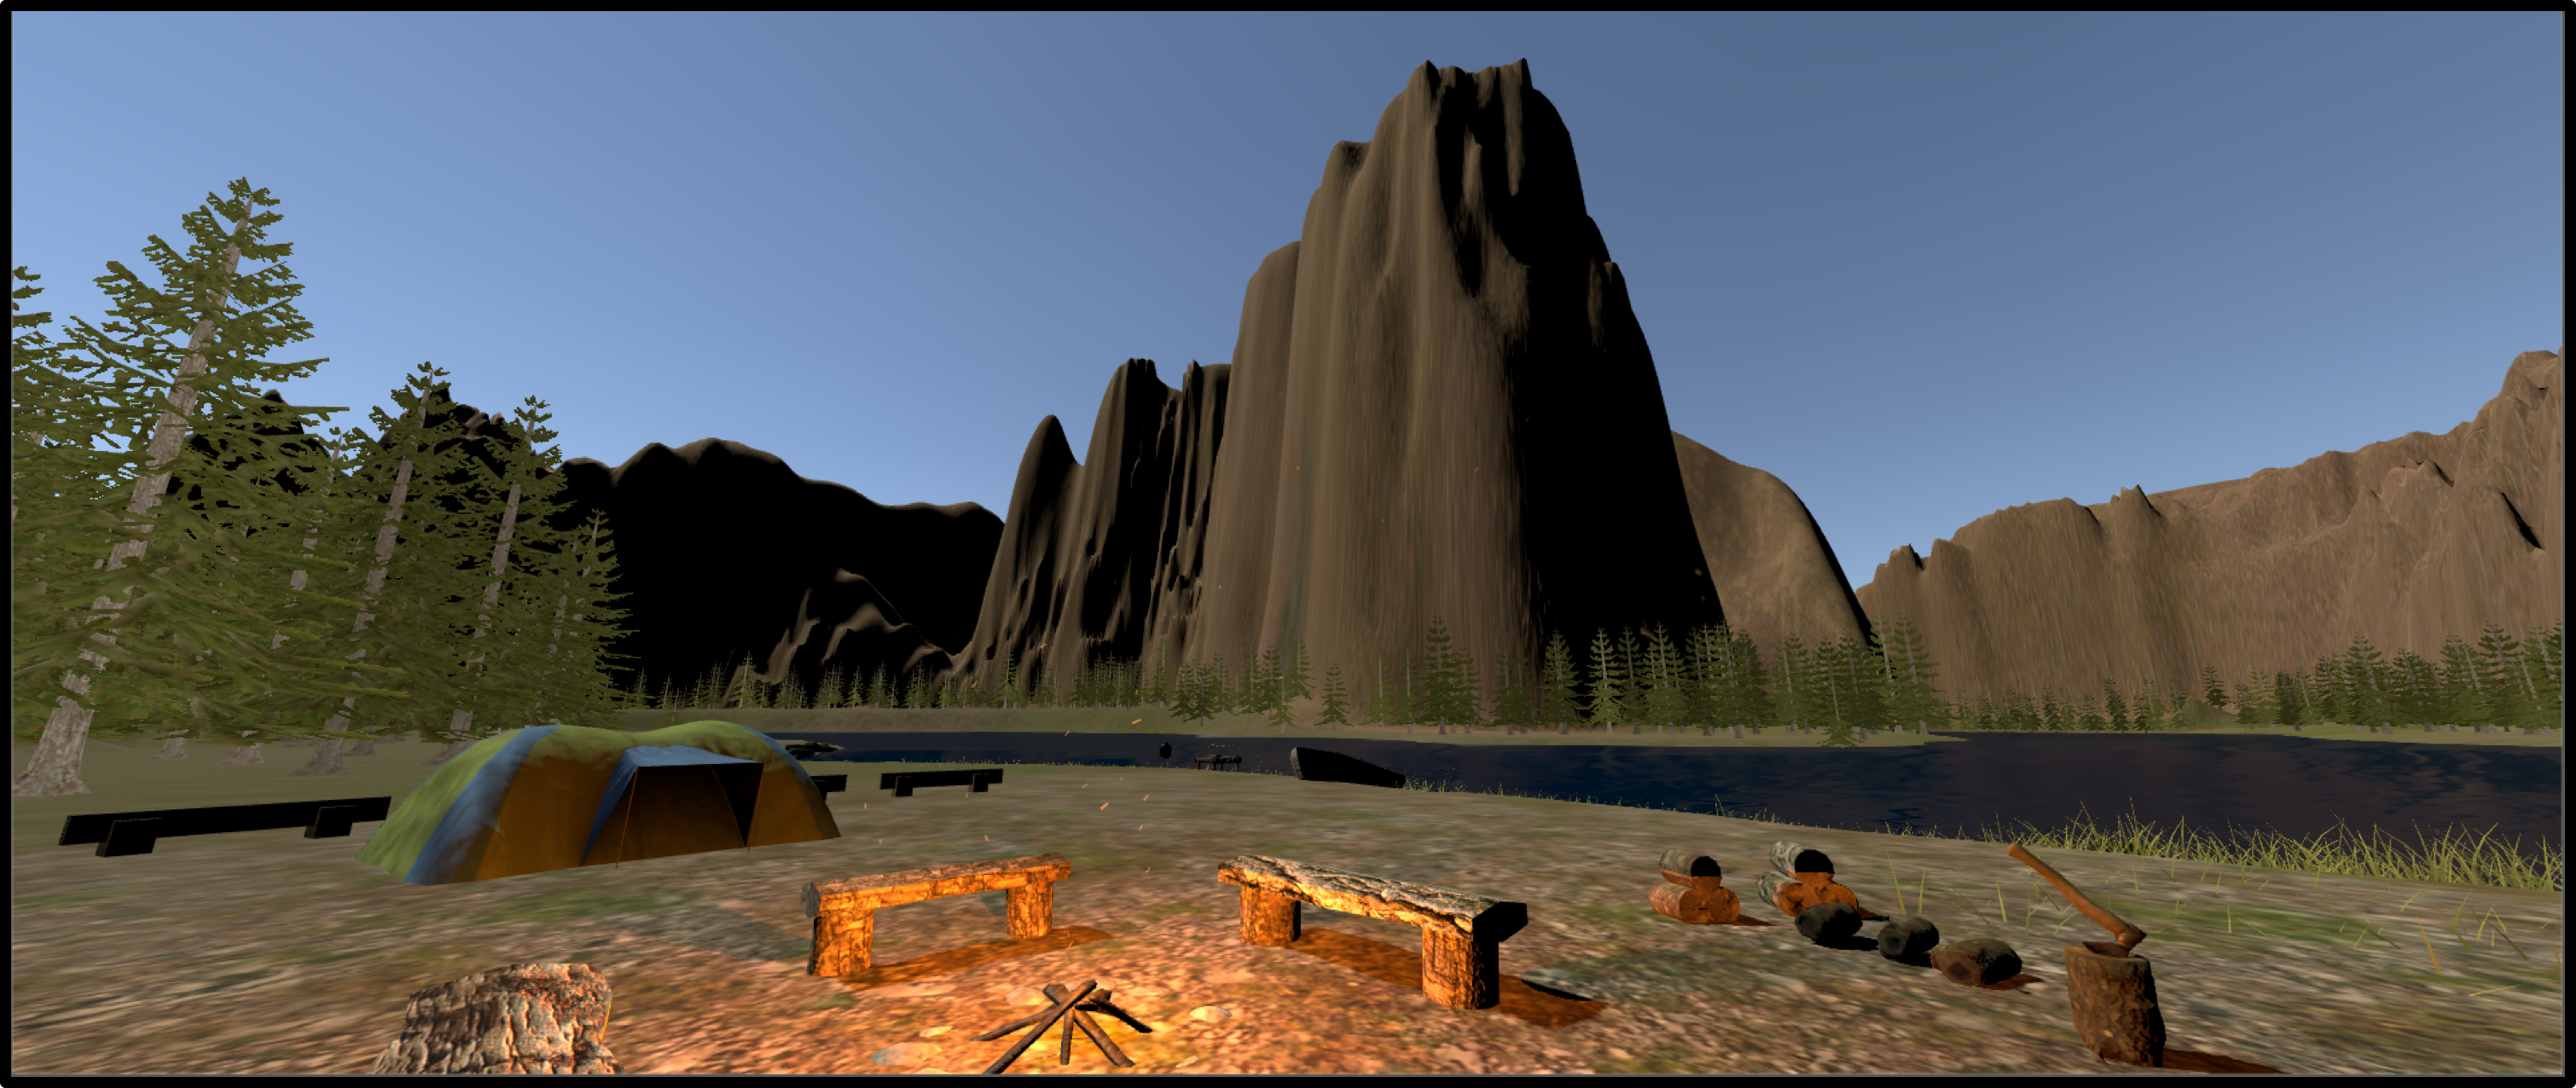
\includegraphics[width=0.80\textwidth]{landscape.png}
    \caption{Image of our landscape}
\end{figure}

\begin{figure}[h]
    \centering
    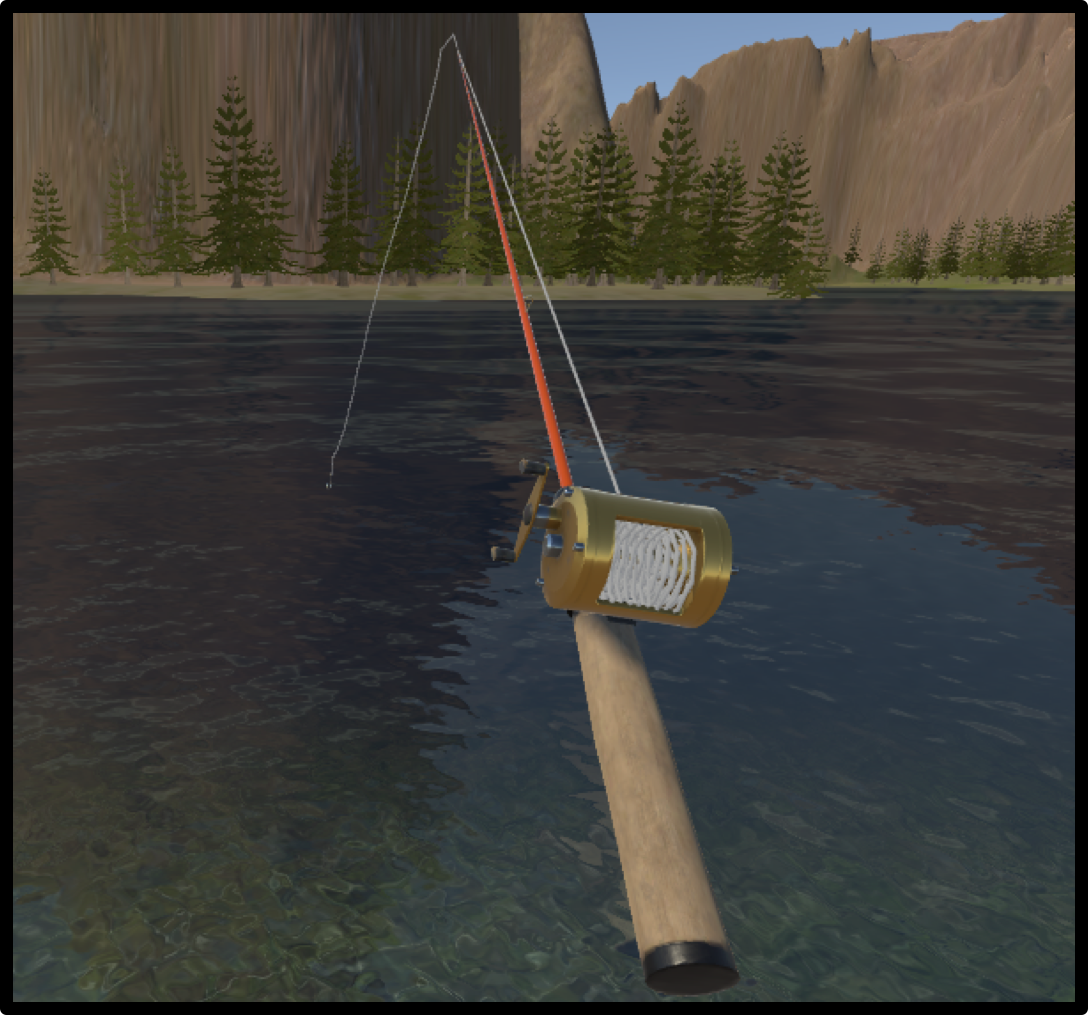
\includegraphics[width=0.5\textwidth]{fishingrod.png}
    \caption{Fishing rod and line}
\end{figure}


\end{document}
